
%%%%%%%%%%%%%%%%%%%%%%%%%%%%%%%%%%%%%%%%%%%%%%
\subsection{Logical View}

Mero is an Exascale ready Object Store system developed by Seagate and built to remove the performance limitations typically found in
other designs. Unlike similar storage systems (e.g., Ceph and DAOS) Mero does
not rely on any other file system or raid software to work. Instead, Mero can
directly access raw block storage devices and provide consistency, durability
and availability of data through dedicated core components. \\

Clovis is the user-space interface exported by Mero for use by the Mero
applications.
Examples of Mero applications are: Mero file system client (m0t1fs), Lustre HSM backend (part of Castor-A200).
ESD middleware will also uses Clovis interfaces to access and manage Mero system.
The logical view for interactions between ESDM and Clovis/Mero is illustrated in \Cref{fig:mero backend logical view}.
 \\
As an object storage, Mero has two types of "objects". In Mero, they are called
Entities, while in object storage, they might be called objects. These
two types of entities are: \\
object, is an array of fixed-size blocks, \\
index, is a key-value store. An index stores records, each record consisting of
       a key and a value. Keys and values within the same index can be of variable
       size. Keys are ordered by the lexicographic ordering of their bit-level
       representation. Records are ordered by the key ordering. Keys are unique
       within an index.\\

Mero defined a set of operations for every type of entities. Mero realm is a
spatial and temporal part of system with a prescribed access discipline.
Objects, indices and operations live in realm. An entity exists in some realm
and has a 128-bit identifier, unique within a Mero cluster and never re-used.
Identifier management is up to the application, except that some identifiers
are reserved for system usage. \\
Generic operations for all entities are: create and delete. They are used to
create a new entity and delete an existing entity. Object has the following
specific operations:
\\
\begin{longtable}{|>{\centering\arraybackslash} m{5.5cm} | >{\centering\arraybackslash} m{6cm} |}\hline\hline
        \cellHeader Mero Object Operation & \cellHeader Description \\ \hline
	READ  & transfer blocks and block attributes from an object to application buffers; \\ \hline
	WRITE & transfer blocks and block attributes from application buffers to an object; \\ \hline
	ALLOC & pre-allocate certain blocks in an implementation-dependent %
                manner. This operation guarantees that consecutive WRITE onto %
                pre-allocated blocks will not fail due to lack of storage space;            \\ \hline
	FREE  & free storage resources used by specified object %
                blocks. Consecutive reads from the blocks will return zeroes.               \\ \hline
        \caption{Mero Object Operations}
\end{longtable}

Index has the following specific operations:
\\
\begin{longtable}{|>{\centering\arraybackslash} m{5.5cm} | >{\centering\arraybackslash} m{6cm} |}\hline\hline
        \cellHeader Mero Index Operation & \cellHeader Description \\ \hline

	GET  &  given a set of keys, return the matching records from the index;    \\ \hline
	PUT  &  given a set of records, place them in the index, overwriting %
	        existing records if necessary, inserting new records otherwise;     \\ \hline
	DEL  &  given a set of keys, delete the matching records from the index;    \\ \hline
	NEXT &  given a set of keys, return the records with the next (in the %
                ascending key order) keys from the index.                           \\ \hline
	LOOKUP  &  given a key, check existence of a record;                        \\ \hline
        \caption{Mero Index Operations}
\end{longtable}



ESD middleware can use Mero indices to store small data and metadata, and objects
to store raw data. For example, Mero indices can be used to keep track of
containers, corresponding variables and shard inside them. Each container will
be represented as an index in Mero. The metadata of this container, the metadata
of all the contained variables, shards and chunks, is stored as key-value records
in this index. Data of variables, shards and chunks can be stored as different
Mero objects. \\

HDF5 file stored in a POSIX file system is identified by its full path name.
ESD middleware needs to keep the mapping from a HDF5 file to Mero identifier of
the index. From this index, ESD middleware can get all metadata for associated
containers and variables and other information. ESD middleware may store the
mapping from HDF5 identity to Mero index identifier in external configuration
storage, e.g. MongoDB, RDBMS, or POSIX file system. Nevertheless, ESD middleware
can also store this mapping in Mero index, too. This index will be a pre-defined
index, with well-known identifier. ESD middleware can initialize this index
at the first of system deployment, and consult it later for this mapping.

\begin{figure}
	\centering
	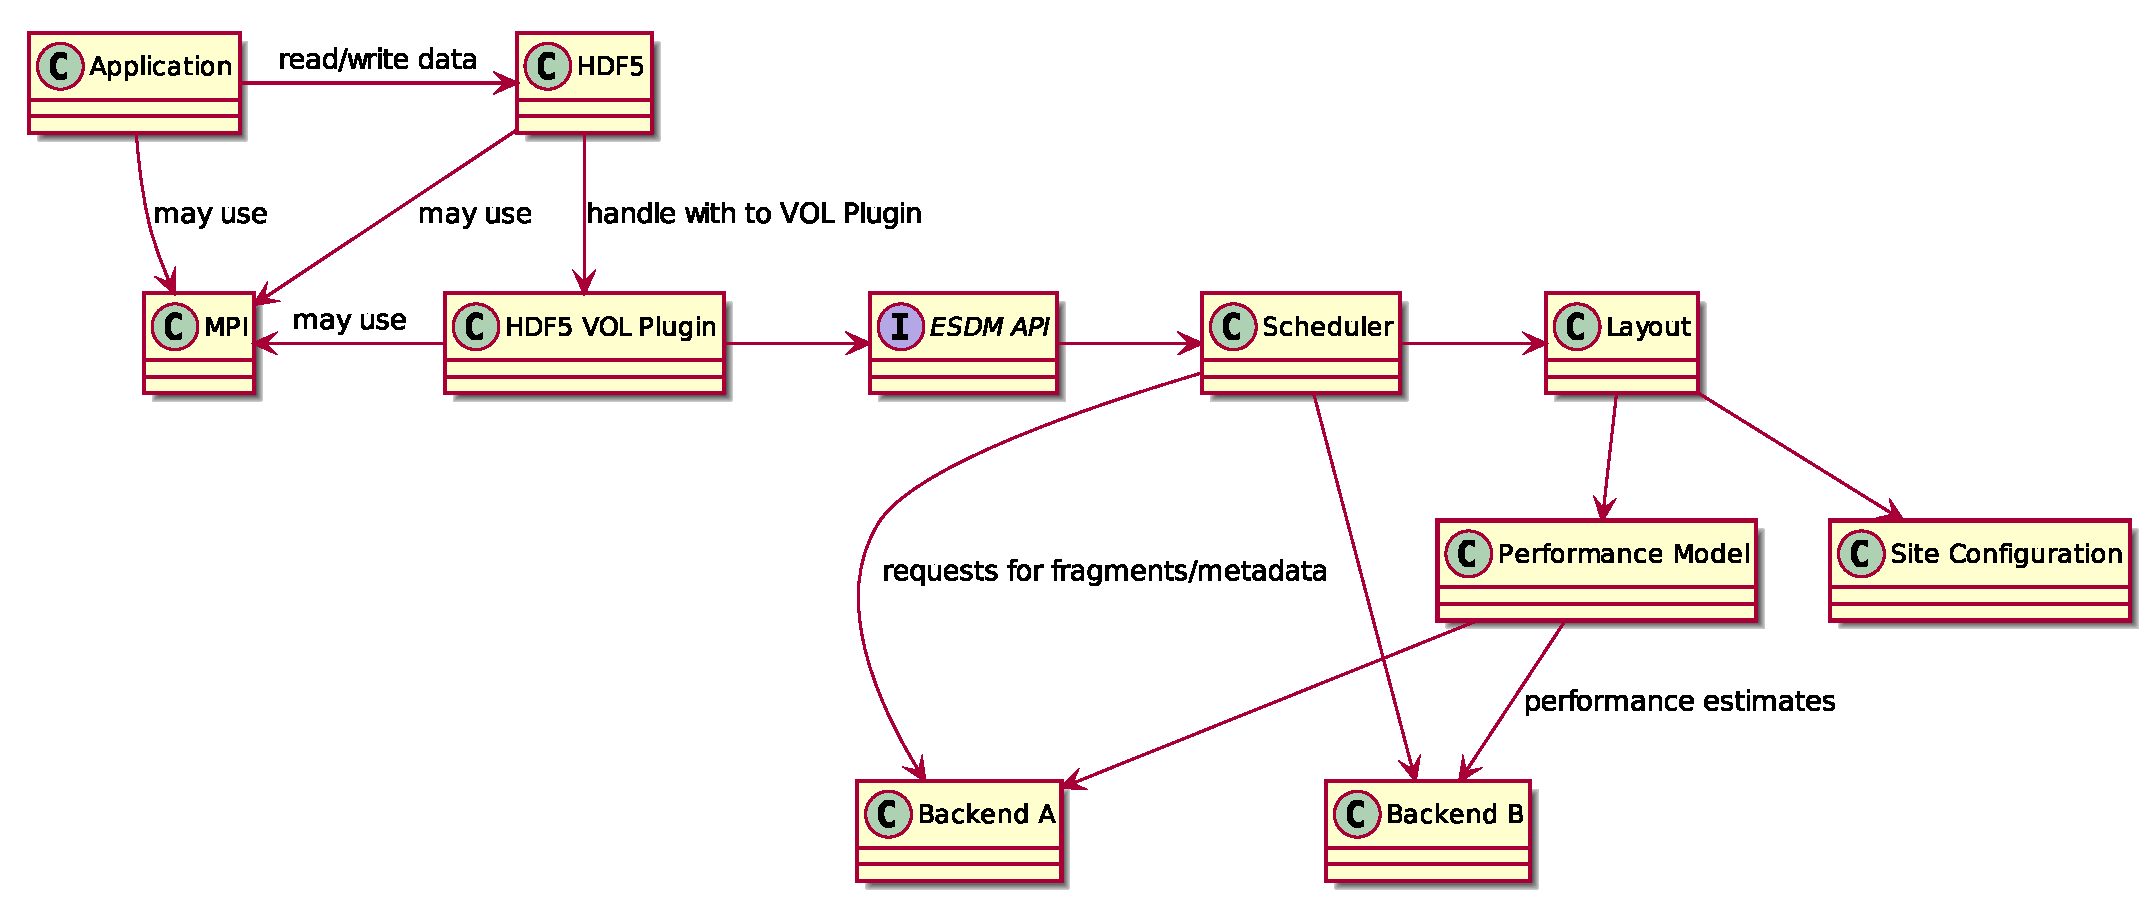
\includegraphics[width=\linewidth]{esdm-backends/mero/logical.eps}
	\caption{Logical view to the Mero backend. I/O requests arrive through the ESDM API. The layout component provides metadata. As a result actual I/O requests are processed by the progress component which calls the backends. The backends and the datatype components work together to convert data according to what is required (again and read and write differ).}
	\label{fig:mero backend logical view}
\end{figure}


\paragraph{Writing data}


The following sequence extends the Use-Case description for general writing
(see \Cref{uc: independent write}).
A sequence diagram for the chain of events is provided by \Cref{fig:mero backend sequence write}.

\begin{itemize}
	\item Progress: consult layout about:
	\begin{itemize}
		\item the identifier(s) of Mero indices to store or update metadata.
		\item the identifier(s) or Mero objects to store or update raw data. %
		      If this is a write to non-exist container, identifiers are generated
		      according to Mero rules.
	\end{itemize}
	\item Progress: if Mero indices/objects don't exist, create them with proper attributes
	\item Progress: GET some records from index if necessary to update some metadata, %
			and prepare metadata to write
	\item Progress: READ blocks from objects if write request is not block-aligned, %
			i.e. partial write. Prepare the in-memory buffer for destination blocks.
	\item Progress: WRITE buffers into blocks of corresponding objects with Mero %
			Clovis object WRITE interface.
	\item Progress: PUT key-value records to index with Mero Clovis index interface.
	\item Progress: Update layout information if necessary
	\item Progress: Wait on Mero back-end until metadata and data are stable on Mero back-end.
	\item Progress: return to upper layer from ESD middleware
\end{itemize}

\begin{figure}
	\centering
	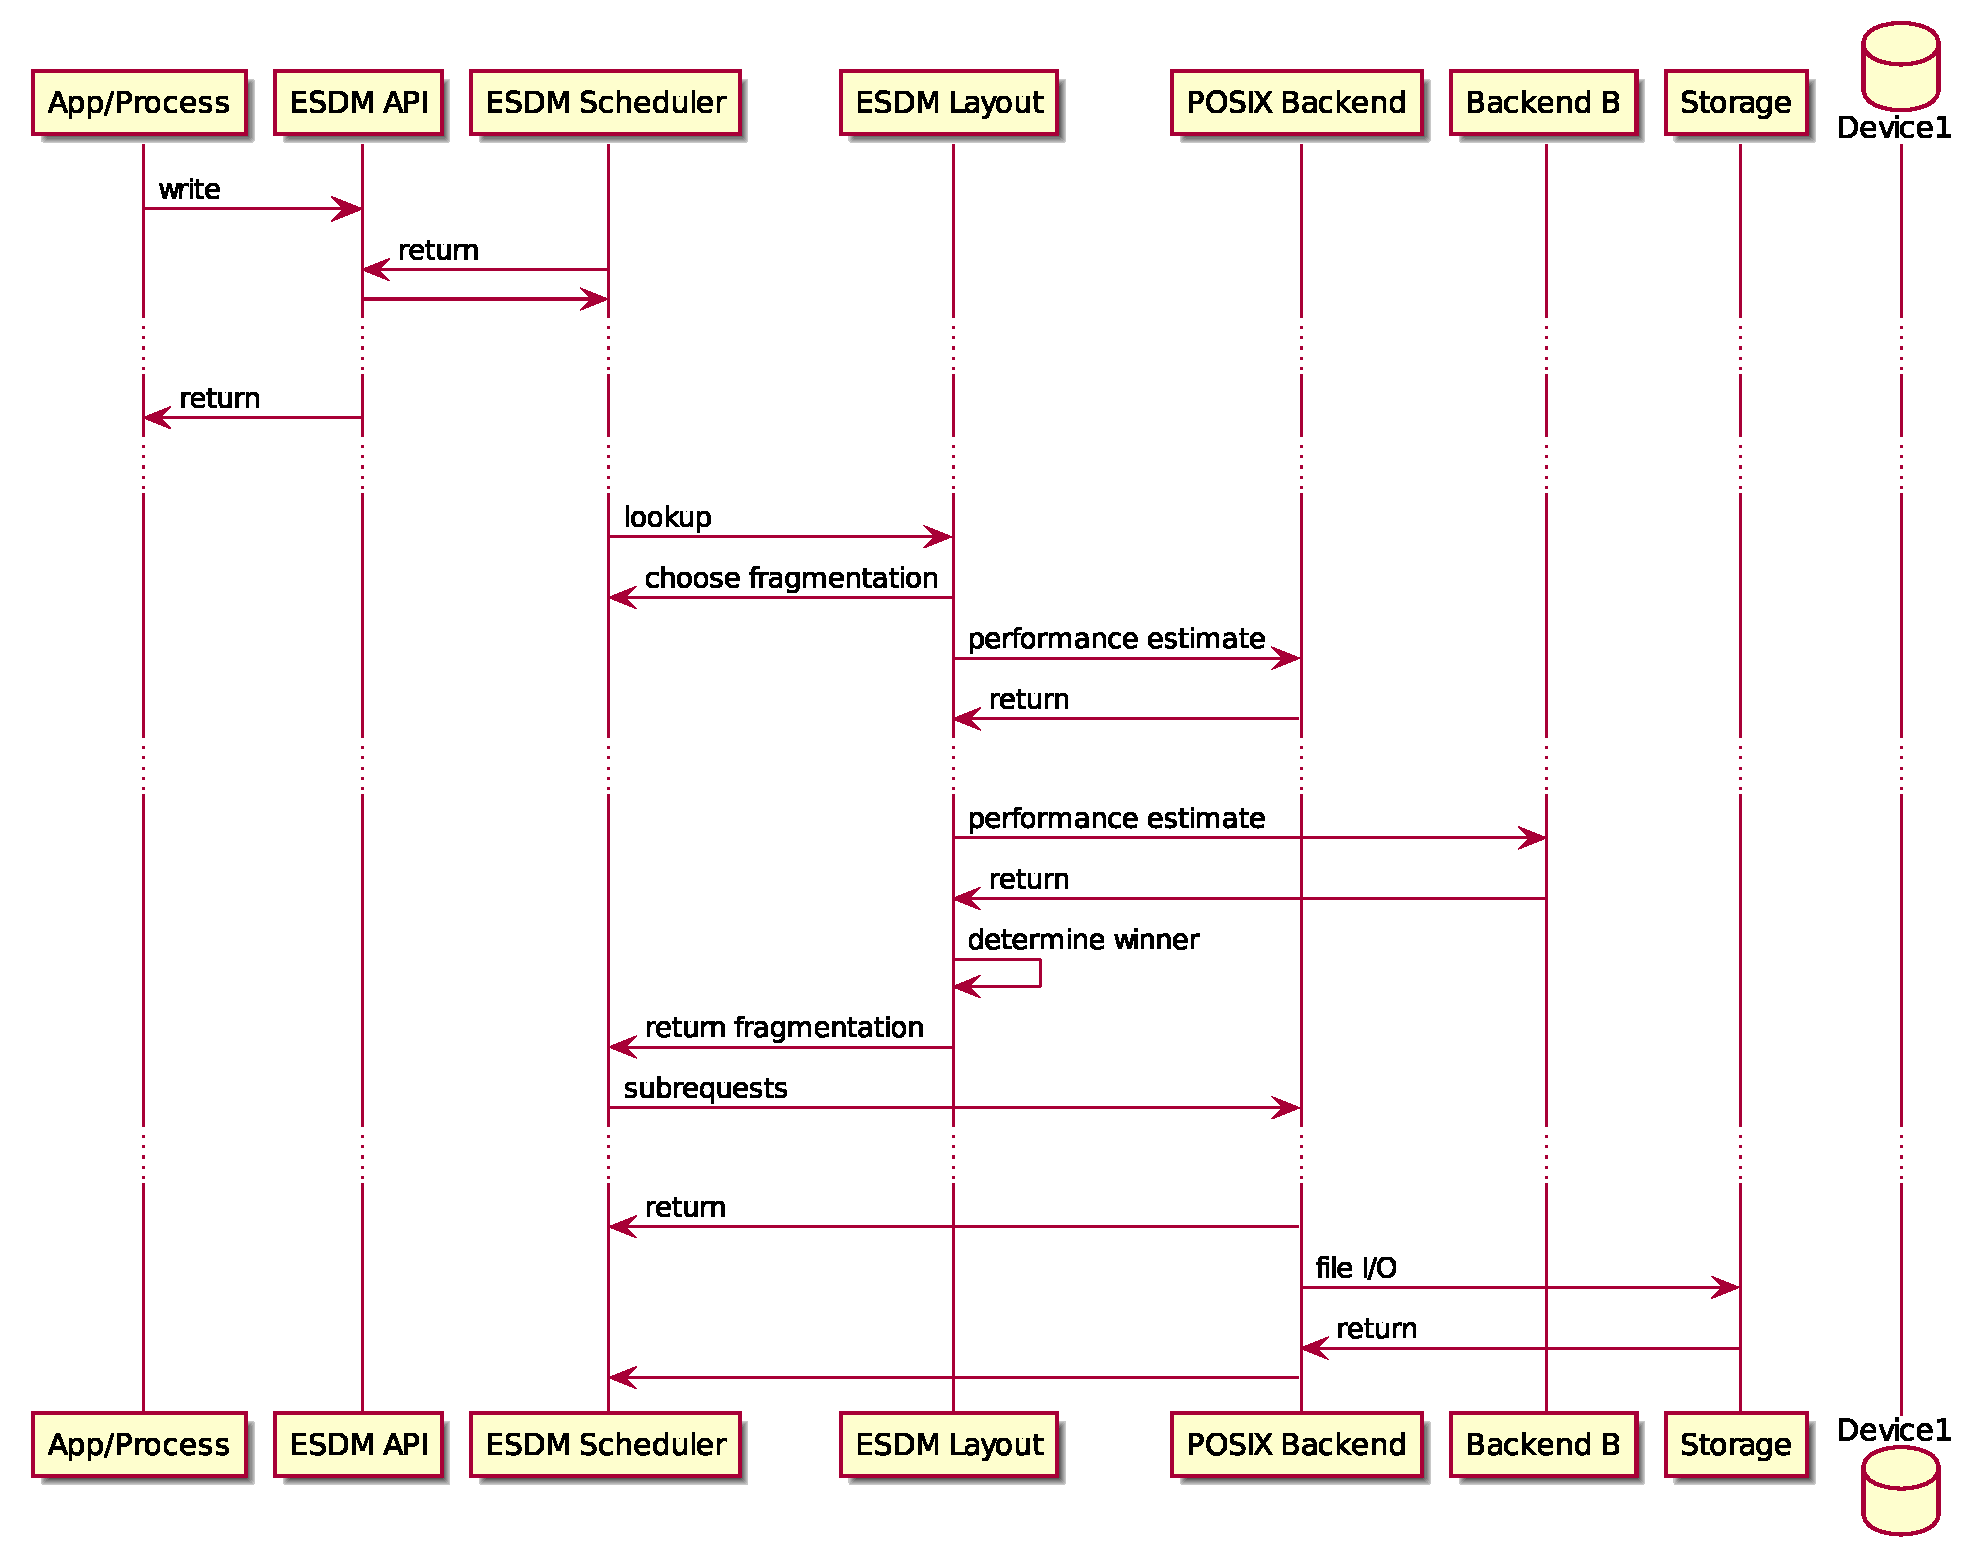
\includegraphics[width=\linewidth]{esdm-backends/mero/sequence_write.eps}
	\caption{Mero backend sequence write}
	\label{fig:mero backend sequence write}
\end{figure}


\paragraph{Reading data}

The following sequence extends the Use-Case description for general reading
(see \Cref{uc: independent read}).
A sequence diagram for the chain of events is provided by \Cref{fig:mero backend sequence read}.

\begin{itemize}
	\item Progress: consult layout about:
	\begin{itemize}
		\item the identifier(s) of Mero indices to store or update metadata.
		\item the identifier(s) or Mero objects to store or update raw data.
	\end{itemize}
	\item Progress: GET necessary key-value records from Mero index and parse the %
			metadata to get information needed by reading.
	\item Progress: With the metadata, layout, mapping the target read to proper object
			and offset blocks.
	\item Progress: READ target blocks from objects, and fill in user buffers.
	\item Progress: return data to upper layer from ESD middleware
\end{itemize}
\begin{figure}
	\centering
	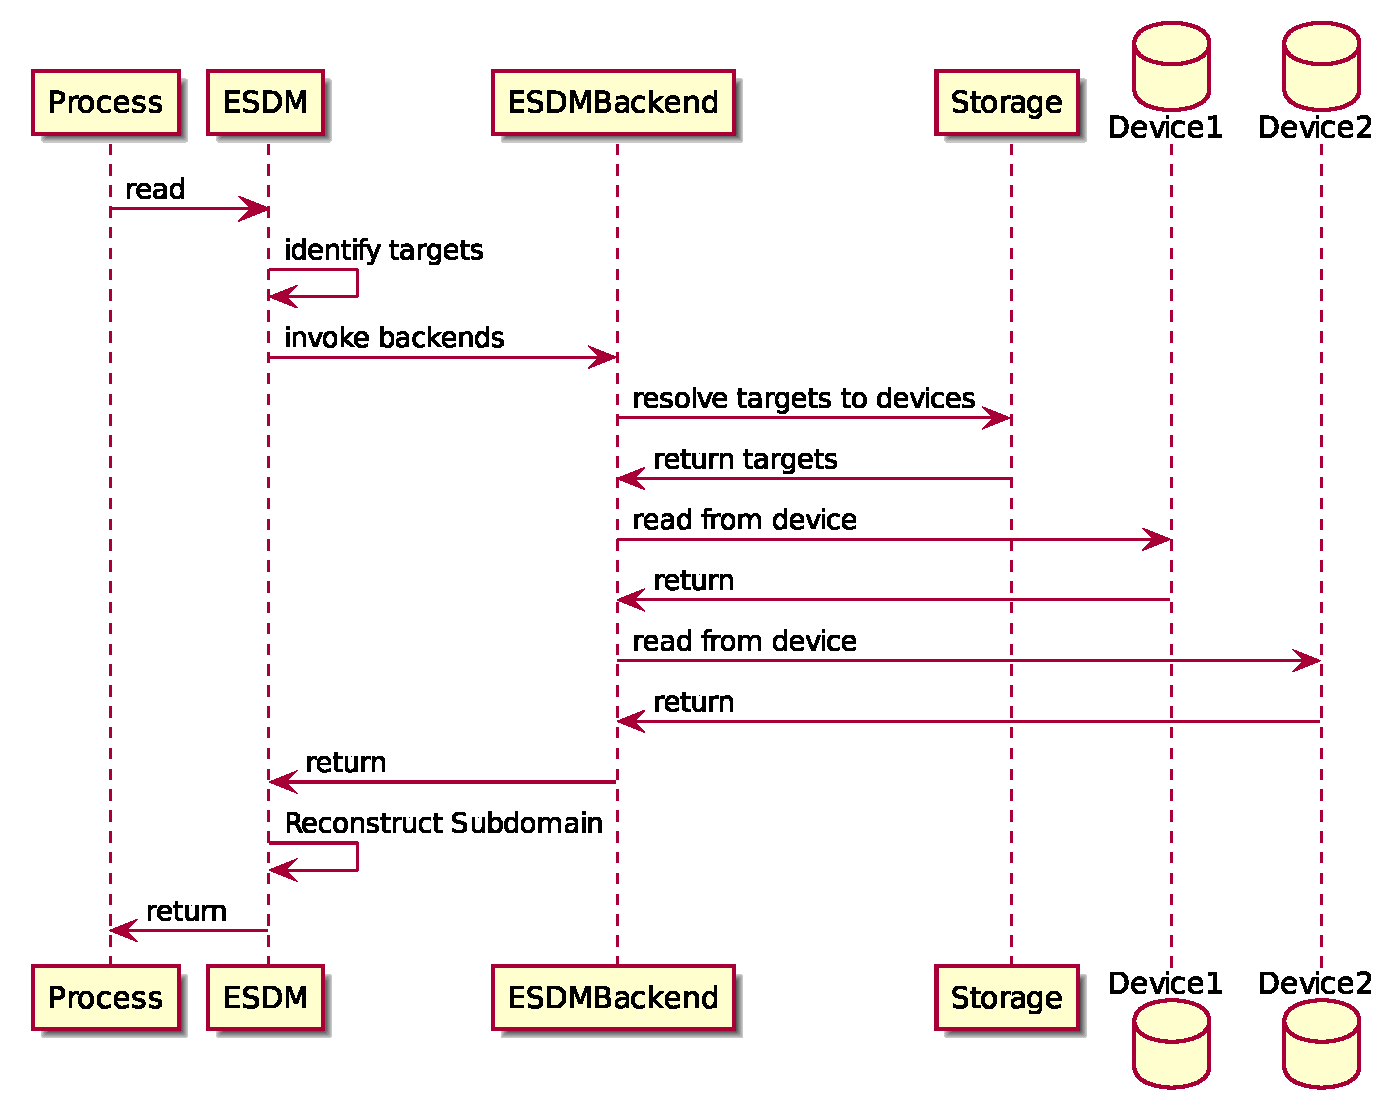
\includegraphics[width=\linewidth]{esdm-backends/mero/sequence_read.eps}
	\caption{Mero backend sequence read}
	\label{fig:mero backend sequence read}
\end{figure}



\paragraph{Lookup:}

The following algorithms are used to store metadata and the steps used to
find out the Mero object blocks mapped to fragments.

On a POSIX file system, a HDF5 file is identified by its full path. On a Mero
back-end, ESD middleware needs to keep the mapping from HDF5 identity to Mero
index identifier. This is a 128-bit integer. All the metadata of this HDF5 are
stored in this Mero index as key-value records. They are: \\
\begin{longtable}{|>{\centering\arraybackslash} m{5.5cm} | >{\centering\arraybackslash} m{6cm} |}\hline\hline
        \cellHeader key & \cellHeader value \\ \hline
	Name           &  String: the name (i.e. identifier)                      \\ \hline
	"ATTR" + Path  &  The attribute of the path. The path is the format of %
			  "/group1/group2/variable\_1". The attribute may be %
			  encoded in some format, e.g. JSON or something. This will %
			  be defined in detailed design.                          \\ \hline
	"OBJ" + Path   &  list of 128-bit identifier of Mero objects %
			  if the variable is stored in a single object, %
			  this would be the only identifier. If the variable %
			  is partitioned into several shards, this would be a list of
			  identifier of Mero object. The shard size and other metadata %
			  would be stored in the above attribute.                  \\ \hline
	Datatype Name  &  Datatype definition in binary mode or string. %
			  This is the named datatype shared by multiple variable.  \\ \hline
	   ...         &   ...                                                     \\ \hline
        \caption{Metadata Schema}
\end{longtable}

The lookup process is to GET all records from Mero index, and parse them to
reconstruct the in-memory metadata.

%%%%%%%%%%%%%%%%%%%%%%%%%%%%%%%%%%%%%%%%%%%%%%
\subsection{Process View}


ESD middleware will use Clovis interfaces to manage and access a Mero cluster.
\Cref{fig:mero backend process view} illustrates the processes and services related to the Mero backend.


\begin{figure}
	\centering
	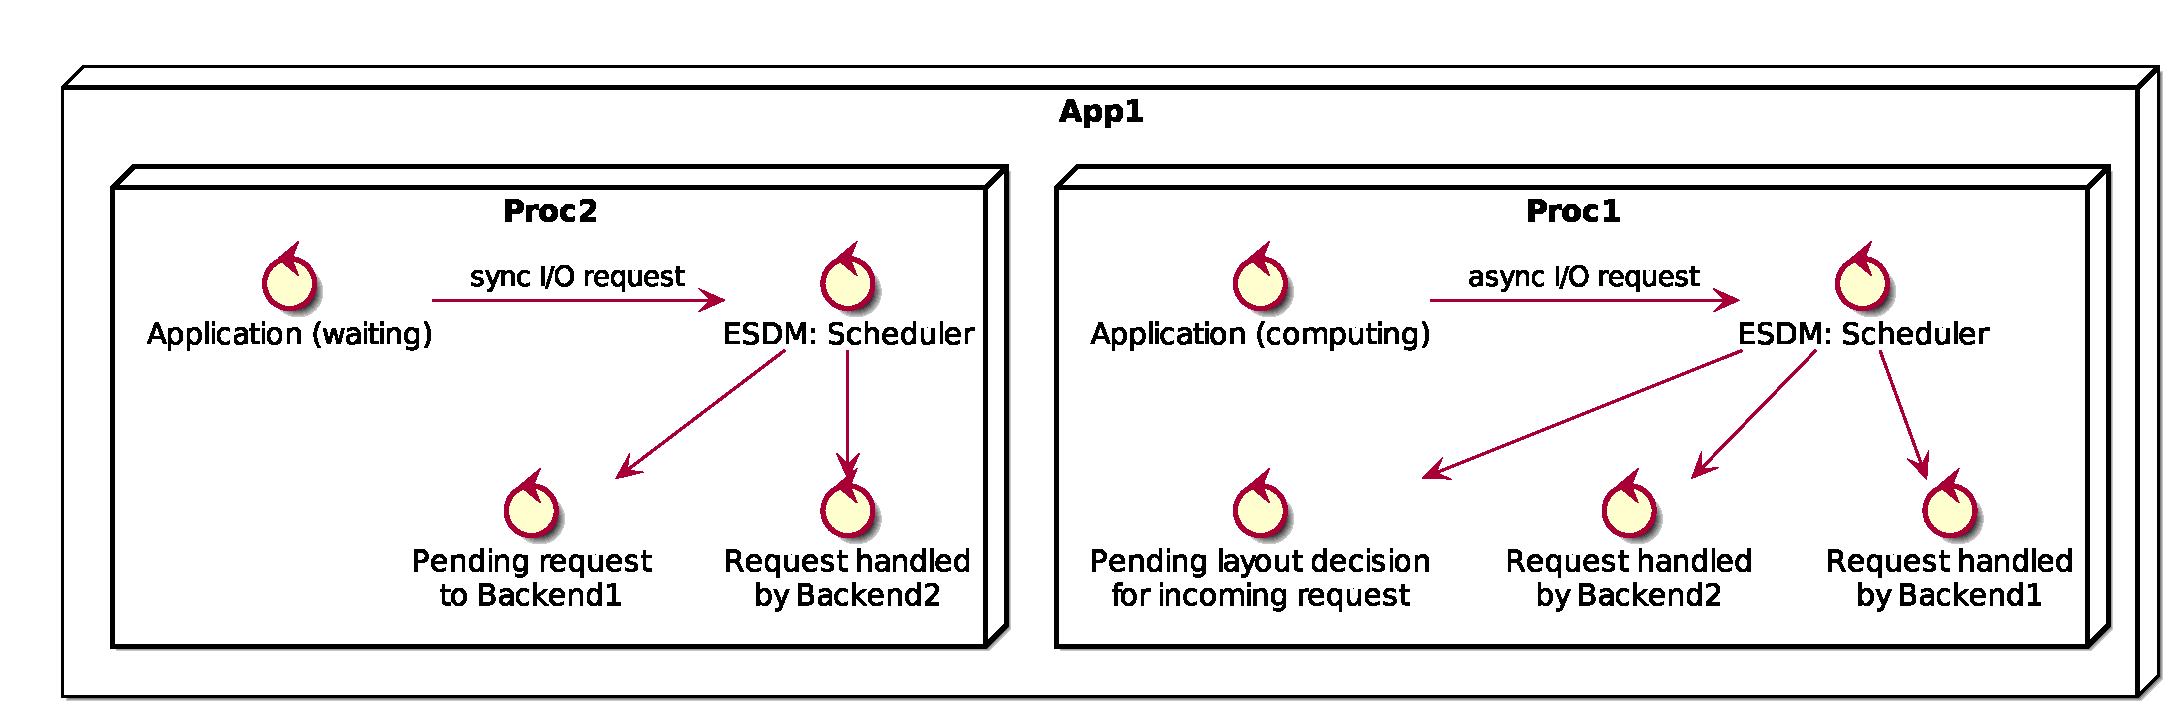
\includegraphics[width=\linewidth]{esdm-backends/mero/process.eps}
	\caption{Overview of processes that are necessary or interact/interfere with the Mero backend.}
	\label{fig:mero backend process view}
\end{figure}

\paragraph{Progress component:}
The progress component is responsible for handling any sync calls as well as
outstanding asynchronous calls that have to be passed to the backend. All Mero Clovis
operations are asynchronous (except for the wait() operations).

\paragraph{Clovis Instance component:}
Clovis instance is a collection of in-memory data structures and their state machines.
ESD middleware keeps a handle to this instance. All communications with Mero
is through this instance. Internally, Clovis uses Mero protocols to communicate with
various Mero services.

\paragraph{Service Management component:}
Mero provides the Clovis interface to manage and access its objects and indices.
Mero also provide a serial of utilities to manage and configure its cluster,
monitor various services, poll system events, and trigger specific operations.
ESD middleware can leverage these interfaces and utilities to communicate with
Mero cluster, and manage all kinds of services and configuration.
\\
The main services
that an application (here is ESD middleware) needs to communicate are:
MeroConfd (configuration and management), MeroRMS (transaction), MeroIOS (index
and object operations).


%%%%%%%%%%%%%%%%%%%%%%%%%%%%%%%%%%%%%%%%%%%%%%
\subsection{Development View}

ESD middleware will use Clovis interfaces to manage and access a Mero cluster.
\Cref{fig:mero backend development view} illustrates the development view of the Mero backend.
ESD middleware code needs to link with Mero Clovis library to access Mero cluster.
Clovis provides interfaces in the C language, currently. All Clovis index and object
operations are asynchronous (except for the wait() operation). A Clovis transaction
is a collection of operations atomic in the face of failures.

\begin{figure}
	\centering
	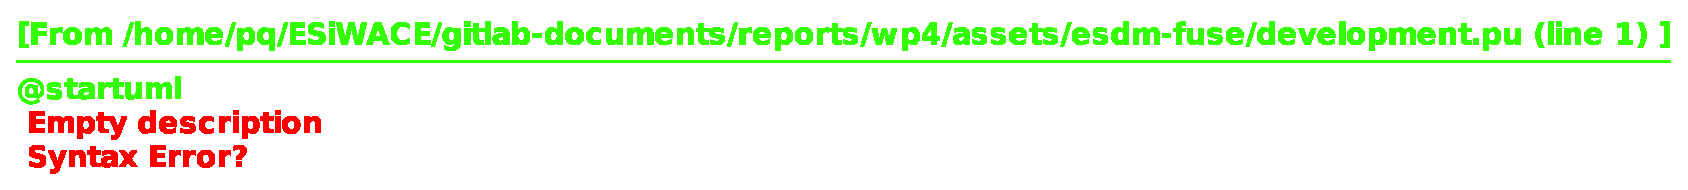
\includegraphics[width=0.25\linewidth]{esdm-backends/mero/development.eps}
	\caption{Development View of Mero backend}
	\label{fig:mero backend development view}
\end{figure}


%%%%%%%%%%%%%%%%%%%%%%%%%%%%%%%%%%%%%%%%%%%%%%
\subsection{Physical View}

Mero storage cluster is relatively an independent system in this case. It can be
managed by Mero utilities. It can also be serving other applications at the
same time. That means, ESD middleware can be one of the applications using
this Mero deployment.
\Cref{fig:backend mero physical view} illustrates the physical view for the Mero backend.

Mero cluster can be configured with different redundant parameters for its
entities. Pool width, [data units, parity units, spare units] for parity
groups of an entity, etc. are those parameters to determine the data redundancy
model, data utilization, performance, and availability. Different configurations
have different mappings from logical data to its physical locations on disks.
But ESD middleware don't have to care about this mapping. ESD middleware uses
Clovis to manage and access Mero entities (Mero indices and objects).
If needed, ESD middleware can use Clovis to create entities with different redundant parameters than the system defaults.

\begin{figure}
	\centering
	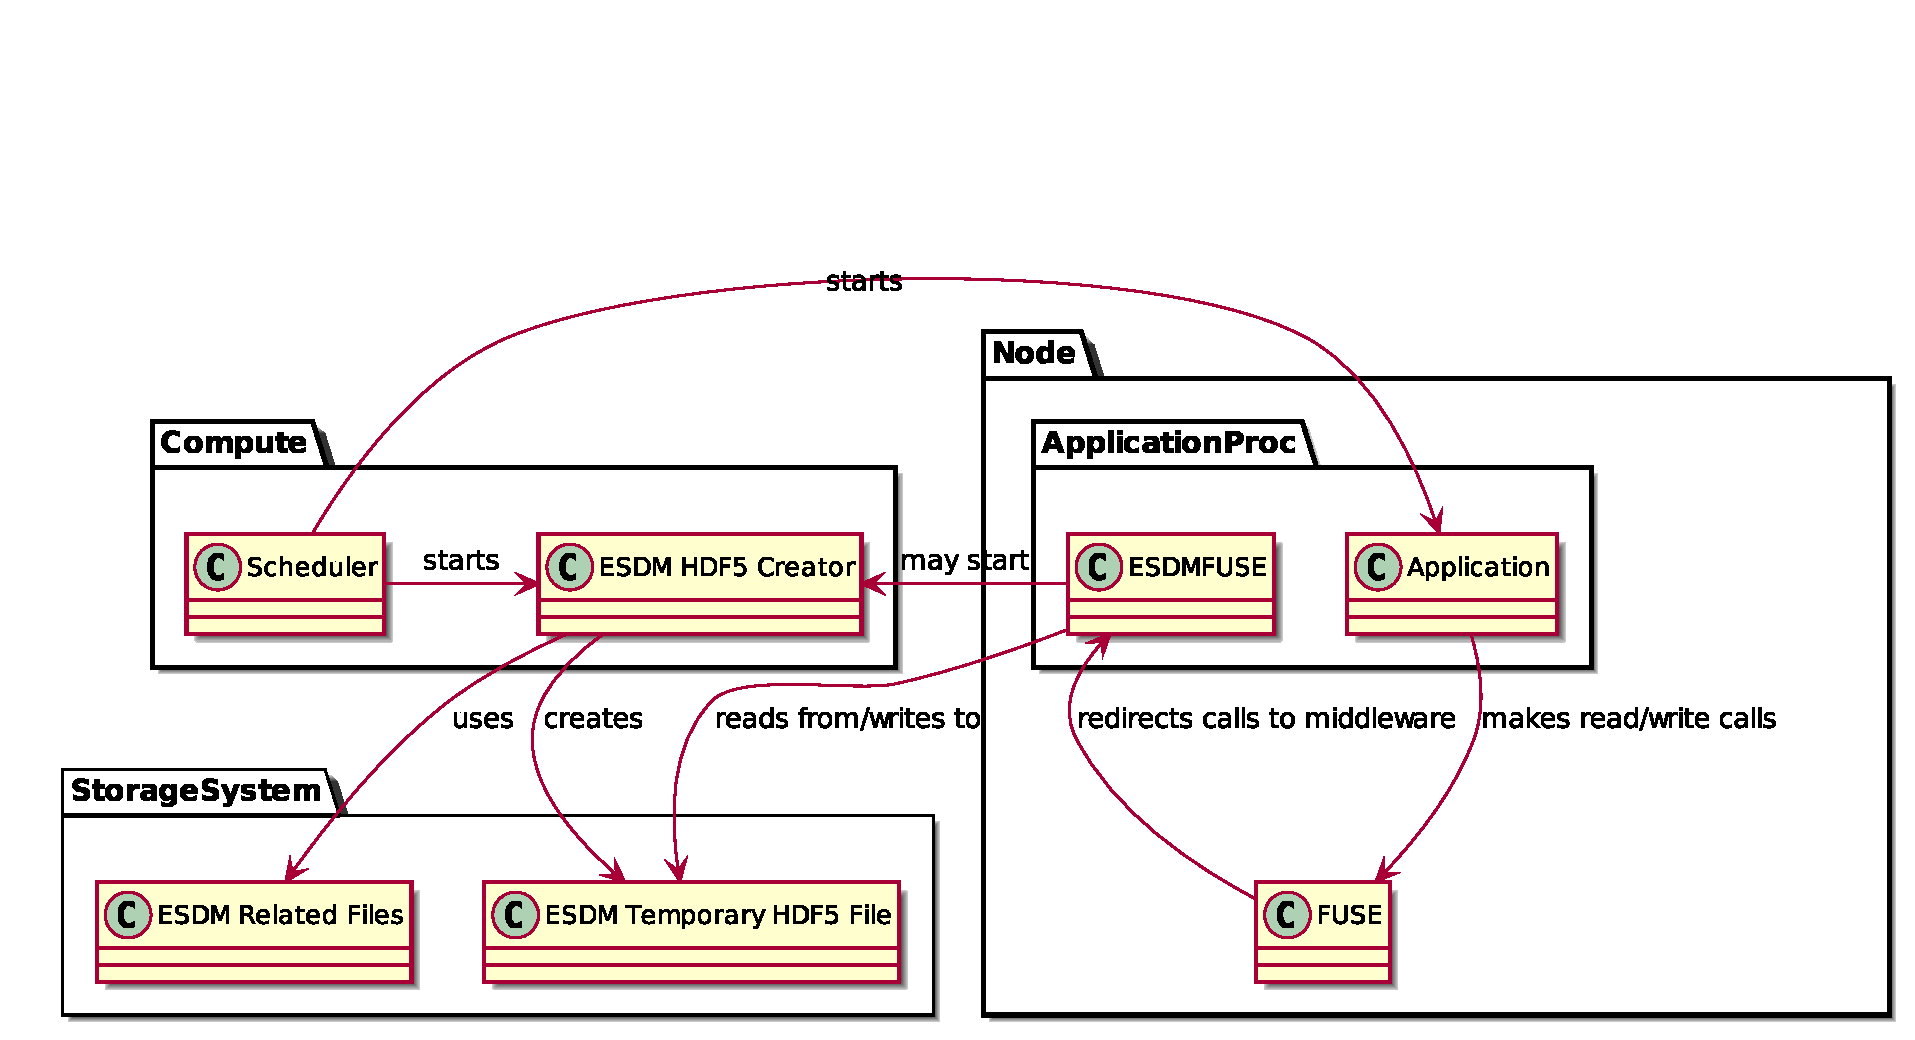
\includegraphics[width=\linewidth]{esdm-backends/mero/physical.eps}
	\caption{Physical mapping of components to location of their execution}
	\label{fig:backend mero physical view}
\end{figure}
